% ### Erste Seite der Schraubverbindungen ###
\centering
\section*{\myul{Schraubverbindungen}}

% Klebefläche für das erste Register:
\begin{tikzpicture}[remember picture, overlay, x=1mm, y=-1mm]
    \begin{scope}[shift={(current page.north west)}]
        \draw (206,56) -- (202,56) -- (202,34) -- (206,34);
        \node[rotate=90, anchor=center] at (204,45) {Schrauben};
    \end{scope}
\end{tikzpicture}

\begin{tikzpicture}[remember picture, overlay]

% --- ERSTE REIHE: Am Seitenursprung anfangen
\setlength{\rowheight}{60mm}

    % X1) Eigene Zeile für die Überschrift
    \Tile{X1}{([xshift=10mm, yshift=-16mm]current page.north west)}{190mm}{8mm}
        {
            \titlebf{Begriffsdefinition}
        }{0}{0}{0}{0}

    % A1) Erste Kachel unten anbauen
    \setlength{\cellwidth}{88mm}
    \Tile{A1}{(X1.south west)}{\cellwidth}{\rowheight}
        {
            \vspace{-\TileSep}
            \titlerm{Verbindungsarten}\\ \vspace{1mm}
            \begin{minipage}[t]{0.5\cellwidth-\TileSep}
                \centering
                \scriptsize
                Durchschraubverbindung (DSV)\\
                Hin{\color{Red}\myul{durchschrauben}}\\
            \end{minipage}%
            \begin{minipage}[t]{0.5\cellwidth-\TileSep}
                \centering
                \scriptsize
                Einschraubverbindung (ESV)\\
                Hin{\color{Red}\myul{einschrauben}}\\
            \end{minipage}\\ \vspace{2mm}
            \begin{minipage}[t]{0.5\cellwidth-\TileSep}
                \centering
                \scriptsize
                Einschraub{\color{Red}en}verbindung\\
                {\color{Red}\myul{Eine}} Schraube\\
            \end{minipage}%
            \begin{minipage}[t]{0.5\cellwidth-\TileSep}
                \centering
                \scriptsize
                Mehrschraub{\color{Red}en}verbindung\\
                {\color{Red}\myul{Mehrere}} Schrauben\\
            \end{minipage}
        }{0}{1}{1}{0}

    % B1) Erste Kachel unten anbauen
    \setlength{\cellwidth}{102mm}
    \Tile{B1}{(A1.north east)}{\cellwidth}{\rowheight}
        {
            \vspace{-\TileSep}
            \titlerm{Belastungen}\\ \vspace{1mm}
            \begin{minipage}[t]{0.55\cellwidth-\TileSep}
                \centering
                \scriptsize
                Längs-/Axialbelastung (Formschluss)\\
                Betriebskraft $F_\text{A}$ in Längsrichtung\\
                Vorspannkraft $F_\text{V}$ der Schraube ({\color{Red}\myul{Lastfrei}})\\
            \end{minipage}%
            \begin{minipage}[t]{0.45\cellwidth-\TileSep}
                \centering
                \scriptsize
                Querbelastung (Reibschluss)\\
                Betriebskraft $F_\text{Q}$ in Querrichtung\\
                Klemmkraft $F_\text{K}$ ({\color{Red}\myul{Betriebsfall}})\\
            \end{minipage}\\ \vspace{2mm}
            \begin{minipage}[t]{0.55\cellwidth-\TileSep}
                \centering
                \scriptsize
                Zentrische Belastung\\
                Längs- / Axialbelastung\\
            \end{minipage}%
            \begin{minipage}[t]{0.45\cellwidth-\TileSep}
                \centering
                \scriptsize
                Exzentrische Belastung\\
            \end{minipage}
        }{0}{0}{1}{0}

% --- ZWEITE REIHE: Unten anbauen
\setlength{\rowheight}{58mm}

    % X2) Eigene Zeile für die Überschrift
    \Tile{X2}{(A1.south west)}{190mm}{7mm}
        {
            \titlebf{Gewindearten}
        }{0}{0}{0}{0}

    % A2) Erste Kachel unten anbauen
    \setlength{\cellwidth}{95mm}
    \Tile{A2}{(X2.south west)}{\cellwidth}{\rowheight}
        {
            \vspace{-\TileSep}
            \resizebox{0.84\cellwidth}{!}{%
            \begin{tabular}{l|l|l}
                \xrowht[()]{1.5mm}\textbf{Bezeichnung} & \textbf{Durchmesser} & \textbf{Fläche} \\ \hline
                \xrowht[()]{5.0mm}\begin{tabular}[c]{@{}l@{}}Außen- /\\[-0.25ex] Nenndurchmesser\end{tabular} & $d$ & $A_\text{N} = \tfrac{\pi~d^2}{4}$ \\ \hline
                \xrowht[()]{3.5mm}\color{NavyBlue}Flankendurchmesser & $d_2 = d - \text{0,64952}\cdot P$ & $A_2 = \tfrac{\pi~d_2^2}{4}$ \\ \hline
                \xrowht[()]{3.5mm}\color{ForestGreen}Kerndurchmesser & $d_3 = d - \text{1,22687}\cdot P$ & $A_3 = \tfrac{\pi~d_3^2}{4}$ \\ \hline
                \xrowht[()]{3.5mm}\color{Red}Spannungsdurchmesser & $d_\text{S} = \text{0,5} \cdot (d_2 + d_3)$ & $A_\text{S} = \tfrac{\pi~d_\text{S}^2}{4}$
            \end{tabular}%
            }%
            \\ \vspace{1mm}
            {\scriptsize($P$ = Gewindesteigung in [mm])}\\ \vspace{1mm}
            \begin{minipage}{0.4\cellwidth-\TileSep}
                \centering
                \vspace{1mm}
                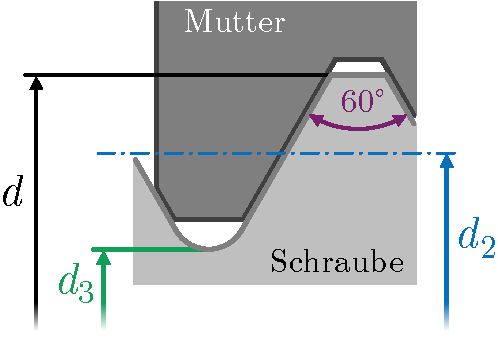
\includegraphics[height=20mm]{images/gewinde-durchmesser-1.pdf}
            \end{minipage}%
            \begin{minipage}{0.3\cellwidth}
                \centering
                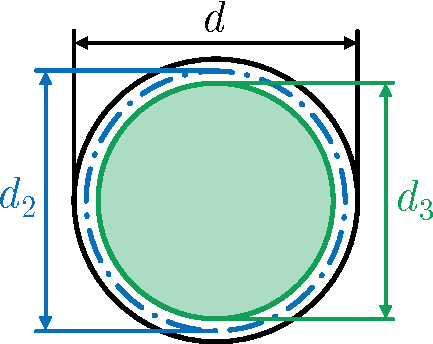
\includegraphics[height=20mm]{images/gewinde-durchmesser-2.pdf}
            \end{minipage}%
            \begin{minipage}{0.3\cellwidth-\TileSep}
                \centering
                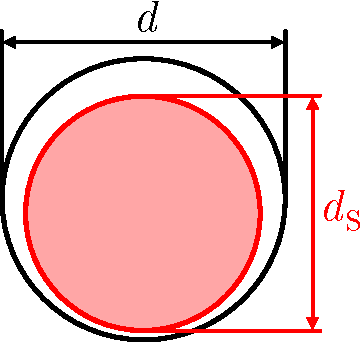
\includegraphics[height=20mm]{images/gewinde-durchmesser-3.pdf}
            \end{minipage}%
        }{0}{1}{1}{0}

    % B2) Erste Kachel unten anbauen
    \setlength{\cellwidth}{95mm}
    \Tile{B2}{(A2.north east)}{\cellwidth}{\rowheight}
        {
            \vspace{-\TileSep}
            \resizebox{\cellwidth-2\TileSep}{!}{%
            \begin{tabular}{l|c|l}
                \xrowht[()]{1.5mm}\textbf{Gewindetyp} & \textbf{Ausführung} & \textbf{Beschreibung} \\ \hline
                \xrowht[()]{7.5mm}Spitzgewinde  & TBD & Übliches Befestigunsgewinde \\
                \xrowht[()]{7.5mm}Trapezgewinde & TBD & \begin{tabular}[c]{@{}l@{}}Bewegungsgewinde\\ (Bsp.: Leitspindeln)\end{tabular} \\
                \xrowht[()]{7.5mm}Rundgewinde   & TBD & \begin{tabular}[c]{@{}l@{}}Bewegungsgewinde für\\ hochverschmutzte Geräte\end{tabular} \\
                \xrowht[()]{7.5mm}Sägegewinde   & TBD & \begin{tabular}[c]{@{}l@{}}Bewegungsgewinde bei\\ einseitiger Belastungsrichtung\end{tabular} \\
                \xrowht[()]{7.5mm}Flachgewinde  & TBD & \begin{tabular}[c]{@{}l@{}}Nicht abgeschrägtes\\ Ineinandergreifen der Zähne\end{tabular}
            \end{tabular}%
            }%
        }{0}{0}{1}{0}

% --- DRITTE REIHE: Unten anbauen
\setlength{\rowheight}{35mm}

    % X3) Eigene Zeile für die Überschrift
    \Tile{X3}{(A2.south west)}{190mm}{7mm}
        {
            \titlebf{Festigkeitsklassen}
        }{0}{0}{0}{0}

    % A3) Erste Kachel unten anbauen
    \setlength{\cellwidth}{190mm}
    \Tile{A3}{(X3.south west)}{\cellwidth}{\rowheight}
        {
            \vspace{-\TileSep}
            \begin{minipage}{0.7\cellwidth-\TileSep}
                \centering
                \begin{tabular}{cclcc|lll}
                    \xrowht[()]{2.0mm}8.8 ($\leq$ M16) & 8.8 ($>$ M16) & 9.8 & 10.9 & 12.9 & \multicolumn{3}{c}{Festigkeitsklasse} \\ \hline
                    \xrowht[()]{2.0mm}640                   & 640                      & 720 & 900  & 1080 & Nennwert       & $R_\text{p0,2}$ & {[}MPa{]}      \\ \cline{1-6}
                    \xrowht[()]{2.0mm}640                   & 660                      & 720 & 920  & 1100 & min.           & $R_\text{p0,2}$ & {[}MPa{]}      \\ \hline
                    \xrowht[()]{2.0mm}800                   & 800                      & 900 & 1000 & 1200 & Nennwert       & $R_\text{m}$    & {[}MPa{]}         \\ \cline{1-6}
                    \xrowht[()]{2.0mm}800                   & 830                      & 900 & 1040 & 1220 & min.           & $R_\text{m}$    & {[}MPa{]}        
                \end{tabular}%
                \\ \vspace{1mm}
                {\scriptsize
                Bei Muttern wird nur die 1. Zahl angegeben.\\[-0.75ex]
                Immer Schrauben und Muttern gleicher Festigkeitsklassen kombinieren!
                }
            \end{minipage}%
            \begin{minipage}{0.3\cellwidth-\TileSep}
                \centering
                \vspace{-5mm}
                \begin{align*}
                    R_\text{m} &= 100\cdot(\text{1.\,Zahl}) \\[1.0ex]
                    R_\text{p0,2} &= \frac{R_\text{m}}{10}\cdot(\text{2.\,Zahl})
                \end{align*}
            \end{minipage}
        }{0}{0}{1}{0}

% --- VIERTE REIHE: Unten anbauen
\setlength{\rowheight}{35mm}

    % X4) Eigene Zeile für die Überschrift
    \Tile{X4}{(A3.south west)}{190mm}{7mm}
        {
            \titlebf{Grobdimensionierung nach VDI 2230}
        }{0}{0}{0}{0}

    % A4) Erste Kachel unten anbauen
    \setlength{\cellwidth}{190mm}
    \Tile{A4}{(X4.south west)}{\cellwidth}{\rowheight}
        {
            \begin{minipage}{0.55\cellwidth-\TileSep}
                \centering
                \setstretch{1.1}
                \begin{enumerate}[leftmargin=*]
                    \item Angreifende Betriebskraft $F_\text{A}$, $F_\text{Q}$ bestimmen
                    \item Wahl der Zeile mit der nächst größeren Kraft $F_\text{A}$, $F_\text{Q}$
                    \item Berücksichtigung der Einbaufälle:\\[1.0ex] \hspace{2mm}
                    \begin{tabular}{lll}
                        Fall 0      & (Axial, Statisch, Zentrisch)    & +\,0 Zeilen \\[0.25ex]
                        Fall I      & (Querkraft, Statisch/Dynamisch) & +\,4 Zeilen \\[0.25ex]
                        Fall II     & (Axial, Dynamisch, Exzentrisch) & +\,2 Zeilen \\[0.25ex]
                        Fall III\,a & (Axial, Dynamisch, Zentrisch)   & +\,1 Zeile  \\[0.25ex]
                        Fall III\,b & (Axial, Statisch, Exzentrisch)  & +\,1 Zeile
                    \end{tabular}
                    \item Ablesen der Mindestvorspannkraft $F_\text{V,\,min}$ (Momentane Zeile)
                    \item Berücksichtigung des Anziehverfahrens:\\[1.0ex] \hspace{2mm}
                    \begin{tabular}{ll}
                        Winkel-/Streckgrenzenkontrolle: & +\,0 Zeilen \\[0.25ex]
                        Drehmomentschlüssel             & +\,1 Zeile  \\[0.25ex]
                        Drehschrauber                   & +\,2 Zeilen
                    \end{tabular}
                    \item Ablesen des Nenndurchmessers $d$ der Schraube, je nach\\[-0.25ex] gewünschter Festigkeitsklasse
                \end{enumerate}
            \end{minipage}%
            \begin{minipage}{0.35\cellwidth-\TileSep}
                \centering
                \resizebox{54mm}{!}{%
                \begin{tabular}{l|r|r|r}
                    \multirow{3}{*}{\begin{tabular}[c]{@{}c@{}}Kraft\\$F_\text{A}$, $F_\text{Q}$ [N]\end{tabular}} & \multicolumn{3}{c}{Nenndurchmesser [mm]}  \\ \cline{2-4}
                                           & \multicolumn{3}{c}{Festigkeitsklasse} \\ \cline{2-4}
                                           & 12.9 & 10.9 & 8.8 \\ \hline
                    250                    & \hspace{8.25mm} & \hspace{8.25mm} & \\ \hline
                    400                    &    &    & \\ \hline
                    630                    &    &    & \\ \hline
                    1.000                  &    &    & \\ \hline
                    1.600                  & 3  & 3  & 3 \\ \hline
                    2.500                  & 3  & 3  & 4 \\ \hline
                    4.000                  & 4  & 4  & 5 \\ \hline
                    6.300                  & 4  & 5  & 5 \\ \hline
                    10.000                 & 5  & 6  & 8 \\ \hline
                    16.000                 & 6  & 8  & 8 \\ \hline
                    25.000                 & 8  & 10 & 10 \\ \hline
                    40.000                 & 10 & 12 & 14 \\ \hline
                    63.000                 & 12 & 14 & 16 \\ \hline
                    100.000                & 16 & 16 & 20 \\ \hline
                    160.000                & 20 & 20 & 24 \\ \hline
                    250.000                & 24 & 27 & 30 \\ \hline
                    400.000                & 30 & 36 & \\ \hline
                    630.000                & 36 &    & 
                \end{tabular}
                }
            \end{minipage}
        }{0}{0}{0}{0}

\end{tikzpicture}

% ### Zweite Seite der Schraubverbindungen ###
\newpage
\centering

\begin{tikzpicture}[remember picture, overlay]

% --- ERSTE REIHE: Am Seitenursprung anfangen
\setlength{\rowheight}{35mm}

    % X1) Eigene Zeile für die Überschrift
    \Tile{X1}{([xshift=10mm, yshift=-9mm]current page.north west)}{190mm}{8mm}
        {
            \titlebf{Schraubenberechnung}
        }{0}{0}{0}{0}

    % A1) Erste Kachel unten anbauen
    \setlength{\cellwidth}{92mm}
    \Tile{A1}{(X1.south west)}{\cellwidth}{\rowheight}
        {
            \vspace{-\TileSep}
            \titlerm{Elastische Längenänderung} {\normalsize$f$ [mm]}\\ \vspace{-2.45mm}
            \begin{equation*}
                f = \varepsilon~l = \frac{l~\sigma}{E} = \frac{F~l}{E~A}
            \end{equation*}%
            \\ \vspace{-4mm}
            \begin{minipage}[t]{0.3\cellwidth-\TileSep}
                \centering
                \scriptsize
                \begin{align*}
                    l           &= \text{Stablänge} \\
                    E           &= \text{E-Modul} \\
                    \sigma      &= \text{Spannung} \\
                    \varepsilon &= \text{Dehnung}
                \end{align*}
            \end{minipage}%
            \begin{minipage}[t]{0.6\cellwidth-\TileSep}
                \centering
                \scriptsize
                \begin{align*}
                    f           &= \text{Elastische Längenänderung} \\
                    F           &= \text{Kraft }(F > 0\text{: Zug; }F < 0\text{: Druck}) \\
                    A           &= \text{Querschnittsfläche}
                \end{align*}
            \end{minipage}
        }{0}{1}{1}{0}

    % B1) Zweite Kachel rechts anbauen
    \setlength{\cellwidth}{98mm}
    \Tile{B1}{(A1.north east)}{\cellwidth}{\rowheight}
        {
            \vspace{-\TileSep}
            \titlerm{Allgemeine Nachgiebigkeit} {\normalsize$\delta$ $\left[\tfrac{\text{mm}}{\text{N}}\right]$}\\ \vspace{-4mm}
            \begin{equation*}
                \delta = \frac{1}{C} = \frac{f}{F} = \frac{l}{E~A}\quad\Rightarrow\quad \delta_i = \sum\limits_{i=1}^n \frac{l_i}{E_\text{s}~A_i}
            \end{equation*}%
            \\ \vspace{-5mm}
            \begin{minipage}[t]{0.35\cellwidth-\TileSep}
                \centering
                \scriptsize
                \begin{align*}
                    \delta &= \text{Nachgiebigkeit} \\
                    l      &= \text{Stablänge} \\
                    E      &= \text{E-Modul} \\
                    A      &= \text{Querschnittsfläche}
                \end{align*}
            \end{minipage}%
            \begin{minipage}[t]{0.60\cellwidth-\TileSep}
                \centering
                \scriptsize
                \begin{align*}
                    f &= \text{Elastische Längenänderung} \\
                    F &= \text{Kraft }(F > 0\text{: Zug; }F < 0\text{: Druck}) \\
                    C &= \text{Federkonstante des Stabs}
                \end{align*}
            \end{minipage}
        }{0}{0}{1}{0}

% --- ZWEITE REIHE: Am Seitenursprung anfangen
\setlength{\rowheight}{82mm}

    % X2) Eigene Zeile für die Überschrift
    \Tile{X2}{(A1.south west)}{190mm}{8mm}
        {
            \titlebf{Spezifische Nachgiebigkeiten}
        }{0}{0}{0}{0}

    % A2) Erste Kachel unten anbauen
    \setlength{\cellwidth}{126mm}
    \Tile{A2}{(X2.south west)}{\cellwidth}{\rowheight}
        {
            \vspace{-\TileSep}
            \titlerm{Schraubennachgiebigkeit} {\normalsize$\delta_\text{S}$ $\left[\tfrac{\text{mm}}{\text{N}}\right]$}\\ \vspace{-3mm}
            \begin{align*}
                \delta_\text{S} &= \frac{f_\text{S}}{F_\text{V}} = \frac{f_\text{A}}{F_\text{AS}} \\[0.75ex]
                                &= \delta_\text{SK} + \delta_1 + \delta_2 +\,\dots\,+ \delta_i + \delta_\text{G} + \delta_\text{M} \\
                                &= \frac{1}{E_\text{S}}\left(\frac{l_\text{SK}}{A_\text{N}} + \frac{l_1}{A_{l_1}} + \frac{l_2}{A_{l_2}} +\,\dots\,+ \frac{l_i}{A_{l_i}} + \frac{l_\text{G}}{A_3} + \frac{l_\text{UG}}{A_3} + \frac{l_\text{M}}{A_\text{N}}\right)
            \end{align*}%
            \\ \vspace{-3mm}
            {\scriptsize
            \begin{align*}
                \delta_i   &= \text{Nachgiebigkeit des Teilquerschnitts }i \\
                E_\text{S} &= \text{Elastizitätsmodul des Schraubenwerkstoffs} \\
                l_i        &= \text{Länge des zylindrischen Einzelelements }i
            \end{align*}
            }\resizebox{\cellwidth-4\TileSep}{!}{%
            \begin{tabular}{llccc}
                \xrowht[()]{1.6mm}Symbol                            & Bezeichnung                        & Fallunterscheidung & Formel                       & Querschnitt                      \\ \hline
                \xrowht[()]{1.6mm}\multirow{2.25}{*}{$l_\text{SK}$} & \multirow{2.25}{*}{eff. Kopflänge} & Außensechskant     & $l_\text{SK}$ = \text{0,5}~d & \multirow{2.25}{*}{$A_\text{N}$} \\
                \xrowht[()]{1.6mm}                                  &                                    & Innensechskant     & $l_\text{SK}$ = \text{0,4}~d &                                  \\ \hline
                \xrowht[()]{1.6mm}$l_\text{G}$                      & eff. Außengewindelänge             &                    & $l_\text{G}$ = \text{0,5}~d  & \multirow{2.25}{*}{$A_3$}        \\
                \xrowht[()]{1.6mm}$l_\text{UG}$                     & ung. Außengewindelänge             &                    & (Rechnen)                    &                                  \\ \hline
                \xrowht[()]{1.6mm}\multirow{2.25}{*}{$l_\text{M}$}  & eff. Mutterlänge                   & DSV                & $l_\text{M}$ = \text{0,4}~d  & \multirow{2.25}{*}{$A_\text{N}$} \\
                \xrowht[()]{1.6mm}                                  & eff. Innengewindelänge             & ESV                & $l_\text{M}$ = \text{0,33}~d & 
            \end{tabular}
            }
        }{0}{1}{1}{0}

    % B2) Zweite Kachel rechts anbauen
    \setlength{\cellwidth}{64mm}
    \Tile{B2}{(A2.north east)}{\cellwidth}{\rowheight}
        {
            \vspace{-\TileSep}
            \titlerm{Plattennachgiebigkeit} {\normalsize$\delta_\text{P}$ $\left[\tfrac{\text{mm}}{\text{N}}\right]$}\\ \vspace{-0.5mm}
            \begin{align*}
                \delta_\text{P} &= \frac{f_\text{P}}{F_\text{V}} = \frac{f_\text{A}}{F_\text{AP}} \\[0.5ex]
                                &= \frac{l_\text{k}}{E_\text{P}~A_\text{ers}}
            \end{align*}%
            \\ \vspace{0.5mm}
            {\scriptsize
            \begin{align*}
                \delta_\text{P} &= \text{Nachgiebigkeit der Platten}             \\
                f_\text{P}      &= \text{Plattenstauchung}                       \\
                F_\text{V}      &= \text{Vorspannkraft}                          \\
                f_\text{A}      &= \text{Längenänderung aufgrund von }F_\text{A} \\
                F_\text{AP}     &= \text{Entlastungskraft der Platten}           \\
                l_\text{k}      &= \text{Klemmlänge}                             \\
                E_\text{P}      &= \text{E-Modul der Platten}                    \\
                A_\text{ers}    &= \text{Ersatzquerschnittsfläche}
            \end{align*}
            }
        }{0}{0}{1}{0}

% --- DRITTE REIHE: Am Seitenursprung anfangen
\setlength{\rowheight}{135mm}

    % A3) Erste Kachel unten anbauen
    \setlength{\cellwidth}{190mm}
    \Tile{A3}{(A2.south west)}{\cellwidth}{\rowheight}
        {
            \titlebf{Ersatzquerschnitt} {\normalsize$A_\text{ers}$ $\left[\text{mm}^2\right]$}\\ \vspace{3mm}
            \begin{tabular}{c|c|c|c|c|c}
                \xrowht[()]{2.5mm}Bedingung & $d_\text{W} \geq D_\text{A}$ & \multicolumn{2}{c|}{$d_\text{W} < D_\text{A} \leq d_\text{W} + l_\text{k}$} & \multicolumn{2}{c}{$D_\text{A} \geq d_\text{W} + l_\text{k}$} \\ \hline
                \xrowht[()]{5.0mm}$A_\text{ers} =$ & $\dfrac{\pi}{4}\left(D_\text{A}^2-d_\text{h}^2\right)$ & \multicolumn{2}{c|}{$\dfrac{\pi}{4}\left(d_\text{W}^2 - d_\text{h}^2\right) + \dfrac{\pi}{8}\,d_\text{W}\left(D_\text{A} - d_\text{W}\right)\left[\left(x+1\right)^2-1\right]$} & \multicolumn{2}{c}{\hspace{5mm}$\dfrac{\pi}{4}\left(d_\text{W}^2 - d_\text{h}^2\right) + \dfrac{\pi}{8}\,d_\text{W}\,l_\text{k}\left[\left(x+1\right)^2-1\right]$}\hspace{4mm} \\ \hline
                \multicolumn{2}{c|}{} & \xrowht[()]{12.0mm}\hspace{7mm}\begin{tabular}[c]{@{}c@{}}DSV:\\[0.5ex]$x = \sqrt[3]{\dfrac{l_\text{k}~d_\text{W}}{D_\text{A}^2}}$\end{tabular}\hspace{7mm} & \begin{tabular}[c]{@{}c@{}}ESV:\\[0.5ex]$x = \sqrt[5]{\dfrac{l_\text{k}}{D_\text{A}}}$\end{tabular} & \hspace{3mm}\begin{tabular}[c]{@{}c@{}}DSV:\\[0.5ex]$x = \sqrt[3]{\dfrac{l_\text{k}~d_\text{W}}{\left(d_\text{W}+l_\text{k}\right)^2}}$\end{tabular}\hspace{3mm} & \begin{tabular}[c]{@{}c@{}}ESV:\\[0.5ex]$x = \sqrt[5]{\dfrac{l_\text{k}}{d_\text{W}+l_\text{k}}}$\end{tabular}
            \end{tabular}%
            \\ \vspace{5mm}
            \begin{minipage}[t]{0.33\cellwidth-\TileSep}
                \centering
                TBD
            \end{minipage}%
            \begin{minipage}[t]{0.33\cellwidth}
                \centering
                TBD
            \end{minipage}%
            \begin{minipage}[t]{0.33\cellwidth-\TileSep}
                \centering
                TBD
            \end{minipage}%
            \\ \vspace{3mm}
            \begin{minipage}[t]{0.3\cellwidth-\TileSep}
                \centering
                \scriptsize
                \begin{align*}
                    A_\text{ers} &= \text{Ersatzquerschnitt}           \\
                    D_\text{A} &= \text{Außendurchmesser der Platten} \\
                    d_\text{W}   &= \text{Durchmesser der Kopfauflage}
                \end{align*}
            \end{minipage}%
            \begin{minipage}[t]{0.3\cellwidth}
                \centering
                \scriptsize
                \begin{align*}
                    l_\text{k} &= \text{Klemmlänge}                       \\
                    d_\text{h} &= \text{Durchmesser des Durchgangsloches} \\
                    x          &= \text{Konstante}
                \end{align*}
            \end{minipage}
            \\ \vspace{3mm}
            {\color{Red}Faustregel:~~$D_\text{A} = 2\cdot\text{Kleinster Randabstand}$}
        }{0}{0}{0}{0}

\end{tikzpicture}